\documentclass[14pt,a4paper]{extarticle}
\usepackage[utf8]{inputenc}
\usepackage[T2A]{fontenc}
\usepackage[english,russian]{babel}
\usepackage{tempora}
\usepackage{geometry}
\geometry{left=30mm,right=15mm,top=20mm,bottom=20mm}
\usepackage{setspace}
\onehalfspacing
\usepackage{indentfirst}
\setlength{\parindent}{1.25cm}
\usepackage{amsmath,amssymb}
\usepackage{graphicx}
\graphicspath{{./}{project/figures/}{figures/}}
\usepackage{float}
\usepackage{booktabs}
\usepackage{longtable}
\usepackage{array}
\usepackage{tabularx}
\usepackage{makecell}
\usepackage{caption}
\usepackage{hyperref}
\hypersetup{unicode=true,colorlinks=false,pdfborder={0 0 0}}
\captionsetup{font=small,labelfont=bf,labelsep=endash}
\renewcommand{\arraystretch}{1.18}
\numberwithin{equation}{section}
\numberwithin{figure}{section}
\numberwithin{table}{section}
\sloppy

\begin{document}
\setcounter{section}{1}

\section{Методология численного моделирования динамики ротора}

\subsection{Цель и задачи расчёта}

Целью расчёта является обеспечение динамических характеристик ротора многоступенчатого центробежного насоса ЦНС 105-392 за счёт корректного учёта гидродинамических сил в подшипниках скольжения и силовых факторов в щелевых уплотнениях.

Для достижения цели решаются следующие задачи:
\begin{itemize}
    \item разработать расчётную схему ротора насоса с сосредоточенными массами рабочих колёс, двумя радиальными опорами и дополнительными радиальными связями от щелевых уплотнений;
    \item выполнить расчёт поля давления в гидродинамическом подшипнике скольжения по уравнению Рейнольдса;
    \item определить полные матрицы жёсткости и демпфирования подшипников с прямыми и перекрёстными коэффициентами;
    \item собрать двумерную балочную модель ротора и определить собственные частоты, формы изгиба и ветви прямой и обратной прецессии;
    \item оценить вынужденные орбиты, перекос шейки в подшипнике и чувствительность результатов к параметрам опор и щелевых уплотнений;
    \item учесть эксплуатационные возмущения: повышенный остаточный дисбаланс, гидродинамическую радиальную силу потока и увеличение зазоров при износе.
\end{itemize}

Для достижения цели рассчитываются поле давления и зазора в подшипнике, динамические коэффициенты $K_{ij}$ и $C_{ij}$, критические скорости, формы изгиба, орбиты центрального и опорных сечений, перекос шейки в подшипнике, а также параметрические зависимости от эксцентриситета, расстояния между опорами и жёсткостных параметров.

\subsection{Расчётная схема насоса}

Объектом расчёта является ротор многоступенчатого секционного насоса ЦНС 105-392, заводское обозначение 5МС-10. Насос имеет восемь рабочих колёс, входной патрубок диаметром $125$ мм и вал с шейкой под подшипник диаметром $90$ мм. Паспортные параметры насоса: подача $Q=105$ м$^3$/ч, напор $H=392$ м, мощность электродвигателя $N=200$ кВт, номинальная частота вращения $n=2950$ об/мин, масса насоса $836$ кг [1]. Требования к насосному оборудованию и общая терминология принимаются с учётом ГОСТ 31381-2009 [2].

Ротор установлен в двух концевых радиальных гидродинамических подшипниках скольжения. По сборочному чертежу и чертежу подшипника стороны всасывания [3] принимаются радиус шейки
\begin{equation}
    R=0{,}045~\text{м}
\end{equation}
и длина рабочей поверхности вкладыша
\begin{equation}
    L_b=0{,}040~\text{м}.
\end{equation}
Материал вкладыша указан как сталь ШХ15 по ГОСТ 801-78 [4]. Радиальный зазор принят по сочетанию посадок $90$H7/e7 для отверстия вкладыша и шейки вала. Для диапазона диаметров $80$--$120$ мм поле H7 даёт отклонения $0\ldots+35$ мкм, а поле e7 для шейки -- примерно $-107\ldots-72$ мкм. Соответственно минимальный, средний и максимальный диаметральные зазоры составляют $72$, $107$ и $142$ мкм, что соответствует среднему радиальному зазору $c=53{,}5$ мкм.

Продольная схема ротора составлена по сборочному чертежу, соответствующему серии 5МС-10 [3]. От центра левой радиальной опоры до начала пакета ступеней принято $0{,}360$ м, длина пакета ступеней -- $1{,}071$ м, расстояние от конца пакета до центра правой радиальной опоры -- $0{,}520$ м. Поэтому расчётный пролёт между центрами радиальных опор равен
\begin{equation}
    l_s=0{,}360+1{,}071+0{,}520=1{,}951~\text{м}.
    \label{eq:span_cns105}
\end{equation}

Восемь рабочих колёс размещаются в пределах пакета ступеней с равным шагом
\begin{equation}
    l_p=\frac{1{,}071}{8}=0{,}133875~\text{м}.
\end{equation}
Координата центра $i$-го рабочего колеса определяется выражением
\begin{equation}
    x_i=0{,}360+\left(i-\frac{1}{2}\right)l_p,\qquad i=1,2,\ldots,8.
    \label{eq:stage_coordinates_cns105}
\end{equation}

По спецификации сборочного чертежа в составе ротора выделяются две позиции рабочих колёс: поз. 12 -- колесо рабочее первой ступени, $1$ шт.; поз. 11 -- рабочее колесо остальных ступеней, $7$ шт. Чертёж колеса первой ступени ЦНС 90.00.00.012 задаёт наружный диаметр $D_2=300$ мм, посадочное отверстие $95$H7, ширину выхода $B_2=22{,}4$ мм, число лопастей $7$, материал Сталь 45 по ГОСТ 1050-88, массу $19{,}6$ кг и допустимый дисбаланс $D_b=250$ г$\cdot$мм [5]. Чертежа колеса поз. 11 в составе исходных данных нет, поэтому его масса принята расчётно: $16{,}0$ кг, что соответствует уменьшению массы примерно на $18\%$ относительно колеса первой ступени за счёт отличия отливки и отсутствия части входных элементов. Последняя ступень отнесена к группе поз. 11, поэтому для неё используется та же расчётная масса $16{,}0$ кг. Суммарная масса восьми рабочих колёс составляет $131{,}6$ кг.

Вал представлен эквивалентной цилиндрической балкой диаметром
\begin{equation}
    d=0{,}090~\text{м}.
\end{equation}
Такой выбор согласован с диаметром шейки подшипника и является консервативным по отношению к участкам вала большего диаметра. Плотность стали принята $\rho=7850$ кг/м$^3$, модуль упругости $E=2{,}1\cdot10^{11}$ Па. Масса участка вала между опорами составляет $97{,}43$ кг, полная расчётная масса ротора с рабочими колёсами -- $229{,}03$ кг.

Расчётная схема ротора приведена на рисунке \ref{fig:rotor_scheme}. На ней показаны сосредоточенные массы рабочих колёс, радиальные опоры, щелевые уплотнения как дополнительные упругие связи, силы тяжести рабочих колёс, сила дисбаланса $F_{\text{д}}$, гидродинамическая радиальная сила потока $F_{\text{г}}$, оси координат и характерный пролёт между опорами.

\begin{figure}[H]
\centering

\includegraphics[width=0.98\textwidth]{06_rotor_scheme_with_seals.png}
\caption{Расчётная схема ротора с рабочими колёсами, радиальными опорами и щелевыми уплотнениями}
\label{fig:rotor_scheme}
\end{figure}

\subsection{Гидродинамическая модель подшипника}

Для определения давления в масляной плёнке используется уравнение Рейнольдса для тонкого слоя вязкой несжимаемой жидкости [6]. В размерной форме для цилиндрического подшипника оно записывается как
\begin{equation}
    \frac{\partial}{\partial x}\left(h^3\frac{\partial p}{\partial x}\right)+
    \frac{\partial}{\partial z}\left(h^3\frac{\partial p}{\partial z}\right)=
    6\eta U\frac{\partial h}{\partial x},
    \label{eq:reynolds_dimensional}
\end{equation}
где $x$ -- координата вдоль окружности подшипника, м; $z$ -- осевая координата, м; $h$ -- толщина смазочного слоя, м; $p$ -- давление, Па; $\eta$ -- динамическая вязкость масла, Па$\cdot$с; $U=\Omega R$ -- окружная скорость шейки, м/с. Вязкость масла в расчёте принята постоянной: $\eta=0{,}01105$ Па$\cdot$с.

Введём безразмерные переменные
\begin{equation}
    \varphi=\frac{x}{R},\qquad Z=\frac{2z}{L_b},\qquad
    H=\frac{h}{c},\qquad P=\frac{p c^2}{2\eta\Omega R^2}.
\end{equation}
Тогда уравнение принимает вид
\begin{equation}
    \frac{\partial}{\partial \varphi}\left(H^3\frac{\partial P}{\partial \varphi}\right)+
    \alpha^2\frac{\partial}{\partial Z}\left(H^3\frac{\partial P}{\partial Z}\right)=
    3\frac{\partial H}{\partial \varphi},
    \qquad \alpha=\frac{2R}{L_b}.
    \label{eq:reynolds_dimensionless}
\end{equation}

Для гладкого цилиндрического подшипника зазор задаётся положением центра шейки. В общем случае малых смещений по двум поперечным направлениям
\begin{equation}
    H(\varphi)=1+\varepsilon_x\cos\varphi+\varepsilon_y\sin\varphi,
    \label{eq:clearance_general}
\end{equation}
где $\varepsilon_x$ и $\varepsilon_y$ -- безразмерные смещения центра шейки, отнесённые к радиальному зазору. В стационарном расчёте несущей способности используется положение $\varepsilon_x=\varepsilon$, $\varepsilon_y=0$:
\begin{equation}
    H_0(\varphi)=1+\varepsilon\cos\varphi.
    \label{eq:clearance_static}
\end{equation}

Граничные условия принимаются периодическими по окружности и нулевыми на торцах вкладыша:
\begin{equation}
    P(0,Z)=P(2\pi,Z),\qquad P(\varphi,-1)=P(\varphi,1)=0.
    \label{eq:boundary_conditions}
\end{equation}
Зона отрицательного давления исключается условием
\begin{equation}
    P_{i,j}=\max(P_{i,j},0),
    \label{eq:cavitation_simple}
\end{equation}
что соответствует инженерному учёту разрыва смазочной плёнки в разгруженной области подшипника.

После решения уравнения Рейнольдса размерные компоненты гидродинамической силы определяются интегрированием давления по поверхности вкладыша:
\begin{equation}
    F_x=S_f\int_{-1}^{1}\int_{0}^{2\pi}P(\varphi,Z)\cos\varphi\,d\varphi\,dZ,
\end{equation}
\begin{equation}
    F_y=S_f\int_{-1}^{1}\int_{0}^{2\pi}P(\varphi,Z)\sin\varphi\,d\varphi\,dZ,
\end{equation}
где масштаб силы равен
\begin{equation}
    S_f=\frac{1}{2}\left(\frac{2\eta\Omega R^2}{c^2}\right)RL_b.
\end{equation}

Рабочий эксцентриситет шейки в каждом подшипнике определяется из статического равновесия, а не задаётся заранее. Сначала по балочной схеме рассчитываются реакции от собственного веса ротора. Для двухопорной балки выполняются условия
\begin{equation}
    W_1+W_2=\sum_j m_jg,\qquad
    W_2 l_s=\sum_j m_jg x_j,
    \label{eq:static_support_reactions}
\end{equation}
где в сумму входят сосредоточенные массы рабочих колёс и распределённая масса вала, приведённая к середине пролёта. Для принятой массовой схемы получены реакции $W_1=1{,}185$ кН и $W_2=1{,}062$ кН. Далее для каждой опоры численно решается уравнение
\begin{equation}
    \left|\mathbf{F}_b(\varepsilon_i)\right|=W_i,
    \label{eq:eccentricity_from_balance}
\end{equation}
где $\mathbf{F}_b(\varepsilon_i)$ -- несущая сила масляной плёнки, полученная интегрированием давления. Получены рабочие эксцентриситеты $\varepsilon_1=0{,}360$ для левой опоры и $\varepsilon_2=0{,}334$ для правой опоры. Среднее значение $\varepsilon=0{,}347$ используется только для иллюстрации поля давления и зазора.

\subsection{Расчёт динамических коэффициентов подшипника}

Линеаризация гидродинамической реакции выполняется в окрестности стационарного положения шейки. Малые изменения силы записываются в форме
\begin{equation}
    \begin{bmatrix}\Delta F_x\\ \Delta F_y\end{bmatrix}=
    \mathbf{K}_b
    \begin{bmatrix}\Delta x\\ \Delta y\end{bmatrix}+
    \mathbf{C}_b
    \begin{bmatrix}\Delta \dot{x}\\ \Delta \dot{y}\end{bmatrix},
    \label{eq:bearing_linear_force}
\end{equation}
где $\mathbf{K}_b$ и $\mathbf{C}_b$ -- матрица опоры по жёсткости и демпфированию:
\begin{equation}
    \mathbf{K}_b=\begin{bmatrix}K_{xx}&K_{xy}\\K_{yx}&K_{yy}\end{bmatrix},\qquad
    \mathbf{C}_b=\begin{bmatrix}C_{xx}&C_{xy}\\C_{yx}&C_{yy}\end{bmatrix}.
    \label{eq:bearing_matrices}
\end{equation}

Коэффициенты находятся численным дифференцированием гидродинамической силы по смещениям и скоростям центра шейки:
\begin{equation}
    K_{ij}=-\frac{\partial F_i}{\partial u_j},\qquad
    C_{ij}=\frac{\partial F_i}{\partial \dot{u}_j},\qquad i,j\in\{x,y\}.
    \label{eq:coefficients_derivatives}
\end{equation}

Матрица опоры не сводится к одному скалярному коэффициенту. Физически это связано с тем, что реакция масляной плёнки не направлена строго противоположно смещению шейки: при вращении вала давление смещается по окружности и возникает составляющая силы, перпендикулярная смещению. Эта составляющая задаёт перекрёстные жёсткости $K_{xy}$, $K_{yx}$ и соответствующие перекрёстные коэффициенты демпфирования. Поэтому гидродинамическая опора описывается несимметричными матрицами коэффициентов, которые передаются в роторную модель без усреднения.

Левая и правая опоры рассчитываются отдельно. Для этого несущая способность подшипника сопоставляется со статическими реакциями опор, после чего для каждой опоры задаётся собственный эксцентриситет. В расчётной схеме используются матрицы $\mathbf{K}_{b1},\mathbf{C}_{b1}$ для левой опоры и $\mathbf{K}_{b2},\mathbf{C}_{b2}$ для правой опоры.

\subsection{Модель упругого ротора}

Ротор моделируется балочными элементами Эйлера--Бернулли. Каждый узел имеет четыре степени свободы
\begin{equation}
    \mathbf{q}_i=\begin{bmatrix}x_i&\theta_{y,i}&y_i&\theta_{x,i}\end{bmatrix}^T,
    \label{eq:node_dofs}
\end{equation}
где $x_i$ и $y_i$ -- поперечные перемещения узла; $\theta_{y,i}$ и $\theta_{x,i}$ -- углы поворота сечений, соответствующие изгибу в двух взаимно перпендикулярных плоскостях.

Матрица жёсткости одного балочного элемента длиной $l_e$ в одной плоскости имеет вид
\begin{equation}
    \mathbf{k}_e=\frac{EI}{l_e^3}
    \begin{bmatrix}
    12&6l_e&-12&6l_e\\
    6l_e&4l_e^2&-6l_e&2l_e^2\\
    -12&-6l_e&12&-6l_e\\
    6l_e&2l_e^2&-6l_e&4l_e^2
    \end{bmatrix},
    \label{eq:beam_stiffness}
\end{equation}
а согласованная матрица масс
\begin{equation}
    \mathbf{m}_e=\frac{\rho A l_e}{420}
    \begin{bmatrix}
    156&22l_e&54&-13l_e\\
    22l_e&4l_e^2&13l_e&-3l_e^2\\
    54&13l_e&156&-22l_e\\
    -13l_e&-3l_e^2&-22l_e&4l_e^2
    \end{bmatrix}.
    \label{eq:beam_mass}
\end{equation}
Эти матрицы собираются независимо для плоскостей $x$ и $y$, а связь между плоскостями вводится через матрицу опоры в концевых подшипниках.

Рабочие колёса учитываются как сосредоточенные массы в поступательных степенях свободы соответствующих узлов. Если $m_i$ -- масса $i$-го рабочего колеса, то в матрицу масс добавляются элементы
\begin{equation}
    M_{x_i x_i}\leftarrow M_{x_i x_i}+m_i,
    \qquad
    M_{y_i y_i}\leftarrow M_{y_i y_i}+m_i.
\end{equation}
В расчёте применяются индивидуальные массы ступеней:
\begin{equation}
    \{m_i\}=\{19{,}60; 16{,}00; 16{,}00; 16{,}00; 16{,}00; 16{,}00; 16{,}00; 16{,}00\}\ \text{кг}.
    \label{eq:stage_masses}
\end{equation}

В опорных узлах в поступательный блок $\{x,y\}$ добавляются матрицы опор. Для левой опоры
\begin{equation}
    \mathbf{K}_{qq}\leftarrow \mathbf{K}_{qq}+\mathbf{K}_{b1},\qquad
    \mathbf{C}_{qq}\leftarrow \mathbf{C}_{qq}+\mathbf{C}_{b1},
\end{equation}
для правой опоры аналогично используются $\mathbf{K}_{b2}$ и $\mathbf{C}_{b2}$.


\subsection{Модель щелевых уплотнений}

Межступенные щелевые уплотнения и щелевое уплотнение разгрузочного устройства учитываются как дополнительные радиальные гидродинамические связи с корпусом. В ротородинамике насосов и турбомашин влияние щелевых уплотнений обычно описывают через радиальные коэффициенты жёсткости и демпфирования [7--12]. Для бакалаврской модели используется инженерная линеаризация эффекта Ломакина [7,8]. Радиальная жёсткость щелевого уплотнения задаётся выражением
\begin{equation}
    K_s=\lambda_L\frac{\gamma_s\Delta p\,D_s L_s}{c_s},
    \label{eq:lomakin_stiffness}
\end{equation}
где $\lambda_L$ -- эмпирический коэффициент; $\Delta p$ -- перепад давления на щелевом уплотнении, Па; $D_s$ -- диаметр уплотнения, м; $L_s$ -- длина уплотнения, м; $c_s$ -- радиальный зазор, м. Демпфирование оценивается через жёсткость
\begin{equation}
    C_s=\beta_s\frac{K_s}{\Omega},
    \label{eq:seal_damping}
\end{equation}
где $\beta_s$ -- безразмерный коэффициент демпфирования.

Для ступеневого щелевого уплотнения перепад давления принят пропорциональным напору одной ступени:
\begin{equation}
    \Delta p_{st}=\gamma_s\frac{\rho_w gH}{z_s},
    \label{eq:stage_pressure_drop}
\end{equation}
где $\rho_w$ -- плотность воды; $H=392$ м -- напор насоса; $z_s=8$ -- число ступеней; $\gamma_s$ -- доля перепада, приходящаяся на щелевое уплотнение. Для переднего щелевого уплотнения рабочего колеса приняты $D_s=110$ мм и $\gamma_s=0{,}40$, для заднего -- $D_s=195$ мм и $\gamma_s=0{,}60$, для щелевого уплотнения разгрузочного устройства -- $D_s=120$ мм и $\gamma_s=0{,}30$. Длина ступеневого уплотнения $L_s=10$ мм находится в диапазоне типовых размеров $8$--$12$ мм, радиальный зазор нового насоса $c_s=0{,}20$ мм находится в диапазоне $0{,}15$--$0{,}25$ мм. Для эксплуатационного увеличения зазора используются значения $0{,}30$--$0{,}40$ мм. В расчёте приняты $\lambda_L=0{,}55$ и $\beta_s=0{,}25$, что соответствует диапазону инженерных оценок для щелевых уплотнений гидравлических машин [7--12]. Переднее и заднее щелевые уплотнения каждого рабочего колеса вводятся отдельными элементами. Щелевое уплотнение разгрузочного устройства расположено со стороны нагнетания.

\subsection{Собственные частоты и орбиты}

После сборки матриц движение ротора описывается системой
\begin{equation}
    \mathbf{M}\ddot{\mathbf{q}}+\mathbf{C}\dot{\mathbf{q}}+\mathbf{K}\mathbf{q}=\mathbf{f}(t).
    \label{eq:rotor_motion}
\end{equation}
Так как матрица опоры содержит перекрёстные компоненты, матрицы $\mathbf{K}$ и $\mathbf{C}$ в общем случае несимметричны. Собственная задача решается в комплексной форме через систему первого порядка
\begin{equation}
    \dot{\mathbf{z}}=\mathbf{A}\mathbf{z},\qquad
    \mathbf{z}=\begin{bmatrix}\mathbf{q}\\\dot{\mathbf{q}}\end{bmatrix},
\end{equation}
\begin{equation}
    \mathbf{A}=\begin{bmatrix}
    \mathbf{0}&\mathbf{I}\\
    -\mathbf{M}^{-1}\mathbf{K}&-\mathbf{M}^{-1}\mathbf{C}
    \end{bmatrix}.
    \label{eq:first_order_matrix}
\end{equation}
Собственные значения $s_j=\sigma_j+i\omega_j$ дают круговые частоты $\omega_j$, частоты в об/мин и знак затухания. Комплексные формы разделяются на ветви прямой и обратной прецессии ротора по фазовому соотношению поперечных перемещений $x$ и $y$.

Вынужденная орбита при синхронном возбуждении определяется в частотной области:
\begin{equation}
    \left(\mathbf{K}-\Omega^2\mathbf{M}+i\Omega\mathbf{C}\right)\mathbf{Q}=\mathbf{F}_0.
    \label{eq:frequency_response}
\end{equation}
Остаточный дисбаланс задаётся по ГОСТ ИСО 1940-1-2007 [14]. Класс точности балансировки определяется произведением допустимого удельного эксцентриситета на угловую скорость, $G=e_{\text{доп}}\Omega$, и имеет размерность мм/с. Физически это величина допустимой остаточной неуравновешенности, отнесённая к скорости точки сечения ротора. В стандарте используются классы от высокоточных G0,4 до грубых G4000. Для газовых турбин применяются классы порядка G2,5, для рабочих колёс центробежных насосов и центрифуг -- G6,3, для роторов промышленного оборудования общего назначения -- G16, а более грубые классы относятся к машинам с невысокими требованиями к вибрации. В расчёте используются G6,3 для нового ротора и G16 для предельно допустимого эксплуатационного состояния.

Допустимый удельный эксцентриситет равен
\begin{equation}
    e_{\text{доп}}=\frac{G}{\Omega}.
    \label{eq:balance_eccentricity}
\end{equation}
Для промежуточного рабочего колеса массой $16{,}0$ кг при $n=2950$ об/мин для класса G6,3 получено $e_{\text{доп}}=20{,}39$ мкм и расчётная сила
\begin{equation}
    F_0=m e_{\text{доп}}\Omega^2=31{,}14~\text{Н}.
    \label{eq:unbalance_force}
\end{equation}
Чертёж колеса первой ступени задаёт независимое ограничение $D_b=250$ г$\cdot$мм. Соответствующая сила при рабочей скорости составляет $23{,}86$ Н, что имеет тот же порядок, что и расчёт по G6,3 для нового ротора.

Если комплексные амплитуды в выбранном сечении равны $Q_x$ и $Q_y$, то траектория центра сечения за период вращения определяется выражениями
\begin{equation}
    x(t)=\operatorname{Re}\{Q_x e^{i\Omega t}\},\qquad
    y(t)=\operatorname{Re}\{Q_y e^{i\Omega t}\}.
    \label{eq:orbit_equations}
\end{equation}
Соотношение полуосей орбиты вычисляется по сингулярным числам матрицы
\begin{equation}
    \mathbf{B}=\begin{bmatrix}
    \operatorname{Re}Q_x&-\operatorname{Im}Q_x\\
    \operatorname{Re}Q_y&-\operatorname{Im}Q_y
    \end{bmatrix}.
    \label{eq:ellipse_axes}
\end{equation}




\subsection{Критерий устойчивости ротора}

Для оценки устойчивости используется тот же комплексный спектр матрицы первого порядка \eqref{eq:first_order_matrix}, который применяется при расчёте собственных частот. Пусть собственное значение системы имеет вид
\begin{equation}
    \lambda_j=\sigma_j+i\omega_j,
\end{equation}
где $\sigma_j=\operatorname{Re}(\lambda_j)$ -- показатель роста или затухания, $\omega_j=\operatorname{Im}(\lambda_j)$ -- круговая частота колебаний. Формальный критерий асимптотической устойчивости линейной системы записывается как
\begin{equation}
    \max_j \operatorname{Re}(\lambda_j)<0.
    \label{eq:stability_real_part}
\end{equation}
При выполнении условия \eqref{eq:stability_real_part} свободные колебания затухают, а при появлении положительной действительной части возникает самовозбуждающаяся ветвь колебаний.

Количественная мера запаса устойчивости для колебательной формы задаётся логарифмическим декрементом
\begin{equation}
    \delta_j=-\frac{2\pi\operatorname{Re}(\lambda_j)}{|\operatorname{Im}(\lambda_j)|}.
    \label{eq:log_decrement}
\end{equation}
Положительный декремент соответствует затухающей форме, а рост $\delta_j$ означает увеличение запаса устойчивости. Для практической интерпретации дополнительно сопоставляются первая частотная ветвь, декременты первых форм и расстояние рабочей скорости от ближайшей критической скорости [11,13].

\subsection{Учёт реальных эксплуатационных нагрузок}

Для расчёта синхронной реакции ротора приняты три силовых варианта. Первый вариант соответствует новому ротору: класс балансировки G6,3 и расчётная гидравлическая радиальная сила потока на номинальном режиме. Второй вариант соответствует допустимому эксплуатационному износу: класс G6,3, повышенная гидравлическая сила при отклонении подачи от номинального режима и увеличение радиального зазора подшипника в $1{,}4$ раза, а зазора щелевых уплотнений -- в $1{,}5$ раза. Третий вариант соответствует предельно допустимому состоянию ротора общего промышленного назначения: класс балансировки G16, повышенная гидравлическая сила и увеличенные зазоры. Класс G16 по ГОСТ ИСО 1940-1-2007 соответствует $e_{\text{доп}}\omega=16$ мм/с и используется как верхняя граница для расчётной проверки ротора [14].

Гидравлическая радиальная сила потока оценивается по инженерной зависимости для центробежных насосов [8,15]
\begin{equation}
    F_{\text{рад}}=K_R\rho_w gH D_2B_2,
    \label{eq:hydraulic_force_stage}
\end{equation}
где $K_R$ -- безразмерный коэффициент радиальной силы; $\rho_w$ -- плотность воды; $H$ -- напор насоса; $D_2=0{,}300$ м -- наружный диаметр рабочего колеса; $B_2=0{,}0224$ м -- ширина выхода колеса по чертежу. В литературе для центробежных насосов коэффициент $K_R$ зависит от режима работы и обычно находится в диапазоне $0{,}02$--$0{,}10$. Для номинального режима принято $K_R=0{,}02$, что даёт $F_{\text{рад}}=516{,}8$ Н. Для нерасчётного режима при отклонении подачи принято $K_R=0{,}04$, что даёт $F_{\text{рад}}=1033{,}7$ Н. В упругой модели эта суммарная сила распределяется по узлам рабочих колёс, а в частотной записи задаётся как синхронная составляющая с неравными проекциями по двум направлениям:
\begin{equation}
    F_x=F_{\text{д}}+F_{\text{рад}},\qquad F_y=-i(F_{\text{д}}+0{,}5F_{\text{рад}}).
    \label{eq:hydraulic_force_components}
\end{equation}

Изменение зазоров при эксплуатации учитывается масштабированием коэффициентов. Для гидродинамического подшипника принято приближение $K_b,C_b\sim c^{-3}$, а для щелевого уплотнения из формулы \eqref{eq:lomakin_stiffness} следует $K_s,C_s\sim c_s^{-1}$. В варианте допустимого износа коэффициенты подшипников пересчитаны для $1{,}4c$, а коэффициенты щелевых уплотнений -- для $1{,}5c_s$. В предельно допустимом варианте используются $1{,}5c$ для подшипников и $2{,}0c_s$ для щелевых уплотнений.

\subsection{Расчёт перекоса шейки}

Перекос шейки в подшипнике оценивается по углам поворота опорного сечения, полученным из гармонической реакции ротора. Для малых углов дополнительное смещение центра шейки вдоль длины вкладыша равно
\begin{equation}
    \Delta e_z=z\theta,
\end{equation}
а безразмерная добавка к эксцентриситету
\begin{equation}
    \Delta\varepsilon_z=\frac{z\theta}{c}.
\end{equation}
Минимальный краевой зазор в наиболее нагруженной стороне вкладыша оценивается как
\begin{equation}
    h_{min,edge}=c\left(1-\varepsilon-\frac{L_b|\theta|}{2c}\right).
    \label{eq:edge_clearance}
\end{equation}
Эта оценка связывает динамическую форму изгиба ротора с локальным режимом работы подшипника. Исследования подшипников с перекосом показывают, что наклон шейки изменяет распределение толщины плёнки и давления, поэтому такой расчёт необходим для проверки эксплуатационного режима [16--18].

\subsection{Выводы по второй главе}

Во второй главе сформулированы цель и задачи расчёта, построена расчётная схема ротора насоса ЦНС 105-392 и задана методика расчёта. Подшипник описывается уравнением Рейнольдса, а его реакция передаётся в роторную модель через матрицу опоры по жёсткости и демпфированию. Ротор собирается в двух плоскостях изгиба, рабочие колёса вводятся индивидуальными массами, щелевые уплотнения учитываются как распределённые радиальные связи. Собственные частоты определяются комплексной задачей первого порядка; по действительным частям собственных значений и логарифмическому декременту выполняется проверка устойчивости. Орбиты рассчитываются по гармонической реакции на остаточный дисбаланс, гидродинамическую силу потока и эксплуатационное увеличение зазоров.

\section{Результаты моделирования}

\subsection{Исходные данные}

Основные параметры расчётной модели приведены в таблице \ref{tab:input_params}. Данные по насосу соответствуют ЦНС 105-392 (5МС-10), а геометрия и масса колеса первой ступени приняты по чертежу ЦНС 90.00.00.012 [1,3,5].

\begin{longtable}{|p{0.22\textwidth}|p{0.18\textwidth}|p{0.16\textwidth}|p{0.32\textwidth}|}
\caption{Исходные данные расчётной модели}\label{tab:input_params}\\
\hline
Параметр & Значение & Единица & Основание выбора \\
\hline
\endfirsthead
\hline
Параметр & Значение & Единица & Основание выбора \\
\hline
\endhead
Марка насоса & ЦНС 105-392, 5МС-10 & -- & Паспортные данные и сборочный чертёж \\
\hline
Подача $Q$ & $105$ & м$^3$/ч & Паспортные данные \\
\hline
Напор $H$ & $392$ & м & Паспортные данные \\
\hline
Мощность & $200$ & кВт & Паспортные данные \\
\hline
Частота вращения & $2950$ & об/мин & Номинальный режим электродвигателя \\
\hline
Число ступеней & $8$ & -- & Паспорт и спецификация насоса \\
\hline
Масса насоса & $836$ & кг & Паспортные данные \\
\hline
Диаметр входного патрубка & $125$ & мм & Сборочный чертёж, соответствие 5МС-10 \\
\hline
Диаметр шейки подшипника & $90$ & мм & Чертёж подшипника \\
\hline
Длина вкладыша & $40$ & мм & Чертёж подшипника \\
\hline
Радиальный зазор & $53{,}5$ & мкм & Среднее значение по посадке H7/e7 сборочного чертежа \\
\hline
Пролёт между опорами & $1{,}951$ & м & Сборочный чертёж \\
\hline
Эквивалентный диаметр вала & $90$ & мм & По шейке подшипника \\
\hline
Колесо первой ступени, поз. 12 & $19{,}60$ & кг & Чертёж детали ЦНС 90.00.00.012 [5] \\
\hline
Колесо промежуточной ступени, поз. 11 & $16{,}00$ & кг & Расчётная оценка по объёму отливки; спецификация сборки [3] \\
\hline
Колесо последней ступени, поз. 11 & $16{,}00$ & кг & Принято как колесо группы поз. 11 по спецификации сборки [3] \\
\hline
Наружный диаметр рабочего колеса $D_2$ & $0{,}300$ & м & Чертёж детали ЦНС 90.00.00.012 [5] \\
\hline
Ширина выхода рабочего колеса $B_2$ & $0{,}0224$ & м & Чертёж детали ЦНС 90.00.00.012 [5] \\
\hline
Допустимый дисбаланс колеса $D_b$ & $250$ & г$\cdot$мм & Чертёж детали ЦНС 90.00.00.012 [5] \\
\hline
Суммарная масса рабочих колёс & $131{,}60$ & кг & $1+7$ колёс по спецификации сборки \\
\hline
Масса вала между опорами & $97{,}43$ & кг & Расчёт по $d=90$ мм и $\rho=7850$ кг/м$^3$ \\
\hline
Полная расчётная масса ротора & $229{,}03$ & кг & Вал и рабочие колёса \\
\hline
Класс балансировки нового ротора & G6,3 & -- & ГОСТ ИСО 1940-1-2007 \\
\hline
Предельно допустимый класс балансировки & G16 & -- & ГОСТ ИСО 1940-1-2007, проверочный расчёт \\
\hline
Длина ступеневого щелевого уплотнения & $10$ & мм & Типовые размеры уплотнений рабочих колёс серии 5МС \\
\hline
Радиальный зазор щелевого уплотнения нового насоса & $0{,}20$ & мм & Типовой диапазон $0{,}15$--$0{,}25$ мм \\
\hline
Переднее щелевое уплотнение рабочего колеса: $D_s;\,\gamma_s$ & $110;\ 0{,}40$ & мм; -- & Геометрия входной зоны колеса и доля перепада давления \\
\hline
Заднее щелевое уплотнение рабочего колеса: $D_s;\,\gamma_s$ & $195;\ 0{,}60$ & мм; -- & Геометрия диска колеса и доля перепада давления \\
\hline
Щелевое уплотнение разгрузочного устройства: $D_s;\,\gamma_s$ & $120;\ 0{,}30$ & мм; -- & Геометрия разгрузочного устройства и доля перепада давления \\
\hline
Коэффициент Ломакина $\lambda_L$ & $0{,}55$ & -- & Диапазон инженерных оценок для щелевых уплотнений \\
\hline
Коэффициент демпфирования щелевого уплотнения $\beta_s$ & $0{,}25$ & -- & Инженерная оценка по модели Ломакина \\
\hline
\end{longtable}

\subsection{Распределение зазора и давления}

Для иллюстрации поля давления используется среднее рабочее значение эксцентриситета $\varepsilon=0{,}347$, полученное из статического равновесия опор. Тогда минимальный зазор в средней плоскости вкладыша составляет $34{,}95$ мкм, максимальный -- $72{,}07$ мкм. Распределение зазора по угловой координате показано на рисунке \ref{fig:clearance}.

\begin{figure}[H]
\centering

\includegraphics[width=0.90\textwidth]{01_clearance_z0.png}
\caption{Распределение безразмерного зазора в средней плоскости подшипника}
\label{fig:clearance}
\end{figure}

Распределение давления в средней плоскости приведено на рисунке \ref{fig:pressure_line}, а двумерное поле давления -- на рисунке \ref{fig:pressure_field}. Давление сосредоточено в сужающейся части зазора. Максимальное давление составляет $0{,}685$ МПа, среднее положительное давление -- $0{,}252$ МПа. Интегральная несущая сила подшипника равна $1{,}102$ кН.

\begin{figure}[H]
\centering

\includegraphics[width=0.90\textwidth]{02_pressure_z0.png}
\caption{Распределение давления в средней плоскости подшипника}
\label{fig:pressure_line}
\end{figure}

\begin{figure}[H]
\centering

\includegraphics[width=0.90\textwidth]{03_pressure_field.png}
\caption{Поле давления в гладком подшипнике}
\label{fig:pressure_field}
\end{figure}

\subsection{Динамические коэффициенты подшипника}

На рисунках \ref{fig:stiffness_coeffs} и \ref{fig:damping_coeffs} показаны зависимости коэффициентов жёсткости и демпфирования от эксцентриситета. При росте эксцентриситета прямая жёсткость $K_{xx}$ увеличивается наиболее быстро, а перекрёстные коэффициенты имеют разные знаки. Это соответствует гидродинамической природе масляной плёнки.

\begin{figure}[H]
\centering

\includegraphics[width=0.90\textwidth]{04_stiffness_coefficients.png}
\caption{Коэффициенты жёсткости гладкого подшипника}
\label{fig:stiffness_coeffs}
\end{figure}

\begin{figure}[H]
\centering

\includegraphics[width=0.90\textwidth]{05_damping_coefficients.png}
\caption{Коэффициенты демпфирования гладкого подшипника}
\label{fig:damping_coeffs}
\end{figure}

Для среднего расчётного положения $\varepsilon=0{,}347$ получены матрицы
\begin{equation}
    \mathbf{K}_{b}=10^6\begin{bmatrix}
    55{,}54&54{,}60\\
    -73{,}62&22{,}53
    \end{bmatrix}\ \text{Н/м},
    \label{eq:k_matrix_result}
\end{equation}
\begin{equation}
    \mathbf{C}_{b}=10^3\begin{bmatrix}
    146{,}24&-493{,}87\\
    -355{,}21&178{,}65
    \end{bmatrix}\ \text{Н}\cdot\text{с/м}.
    \label{eq:c_matrix_result}
\end{equation}
Для левой опоры из уравнения статического равновесия получен эксцентриситет $\varepsilon_1=0{,}360$, для правой -- $\varepsilon_2=0{,}334$. Соответственно средние прямые жёсткости левой и правой опор составляют $41{,}6$ и $36{,}6$ МН/м.

\subsection{Расчёт критических скоростей}

Сначала рассчитана модель без щелевых уплотнений, в которой действуют только концевые подшипники с матрицей опоры. Первые две комплексные ветви составили $1629{,}3$ и $1634{,}2$ об/мин. Близость этих частот показывает разделение первой пары на ветви обратной и прямой прецессии.

После введения межступенных щелевых уплотнений и щелевого уплотнения разгрузочного устройства первая пара сместилась до $3701{,}8$ и $3705{,}7$ об/мин. Третья ветвь находится на уровне $8467{,}7$ об/мин. В предельно допустимом варианте с увеличенными зазорами первая пара составляет $2900{,}0$ и $2901{,}6$ об/мин. Номинальная рабочая скорость $2950$ об/мин находится немного выше расчётной первой ветви для предельно допустимого состояния, поэтому такой вариант следует рассматривать как граничный по вибрационной надёжности.

На рисунке \ref{fig:first_mode} приведена первая нормированная форма изгиба. В модели без щелевых уплотнений пучность формы расположена около $x=0{,}962$ м. При учёте щелевых уплотнений пучность смещается к $x=0{,}829$ м, а при увеличенных зазорах -- к $x=0{,}871$ м.

\begin{figure}[H]
\centering

\includegraphics[width=0.90\textwidth]{07_first_mode_shape_seals_comparison.png}
\caption{Первая нормированная форма изгиба ротора}
\label{fig:first_mode}
\end{figure}

На рисунке \ref{fig:critical_comparison} сопоставлены жёсткая оценка, модель без щелевых уплотнений, модель с номинальными щелевыми уплотнениями и изношенный вариант. Жёсткая оценка завышает первую частоту, так как не учитывает изгибную податливость длинного вала.

\begin{figure}[H]
\centering
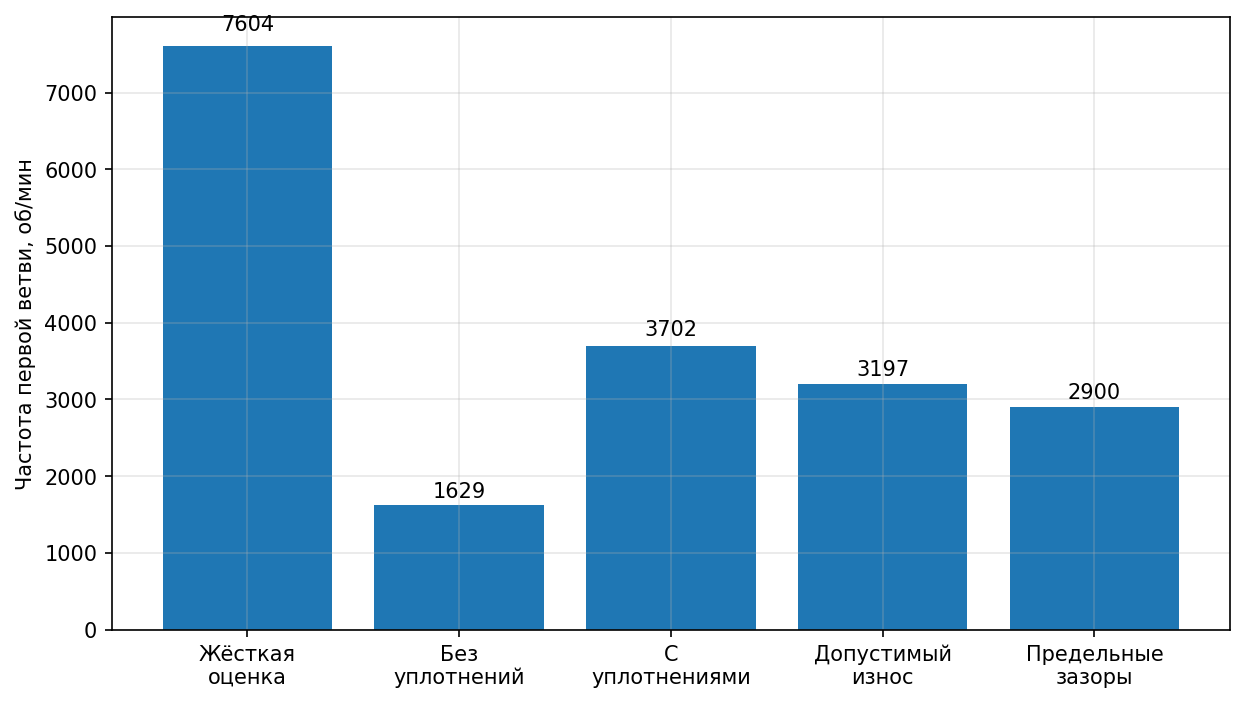
\includegraphics[width=0.85\textwidth]{08_critical_speed_comparison_seals.png}
\caption{Сравнение первой частотной ветви для расчётных вариантов}
\label{fig:critical_comparison}
\end{figure}

Суммарная жёсткость шестнадцати ступеневых щелевых уплотнений равна $17{,}0$ МН/м, а жёсткость щелевого уплотнения разгрузочного устройства -- $17{,}1$ МН/м. Эти значения меньше жёсткости концевых подшипников, однако их влияние существенно из-за распределения вдоль пакета ступеней. Сопоставление вкладов показано на рисунке \ref{fig:seal_contrib}.

\begin{figure}[H]
\centering

\includegraphics[width=0.85\textwidth]{15_seal_stiffness_contributions.png}
\caption{Сопоставление средней прямой жёсткости опор и щелевых уплотнений}
\label{fig:seal_contrib}
\end{figure}



\subsection{Расчёт орбит}

Для нового ротора при классе G6,3 с номинальной гидравлической радиальной силой полуоси орбиты центрального сечения равны $51{,}60$ и $26{,}95$ мкм. В варианте допустимого эксплуатационного износа при том же классе балансировки, повышенной гидравлической силе и увеличенных зазорах полуоси составляют $252{,}20$ и $121{,}03$ мкм. В предельно допустимом варианте G16 с увеличенными зазорами полуоси возрастают до $488{,}38$ и $285{,}49$ мкм. Амплитуды синхронных сил в этих вариантах составляют соответственно $|F_x|=548{,}0$ Н и $|F_y|=289{,}6$ Н, $|F_x|=1064{,}8$ Н и $|F_y|=548{,}0$ Н, $|F_x|=1112{,}8$ Н и $|F_y|=595{,}9$ Н.

\begin{figure}[H]
\centering
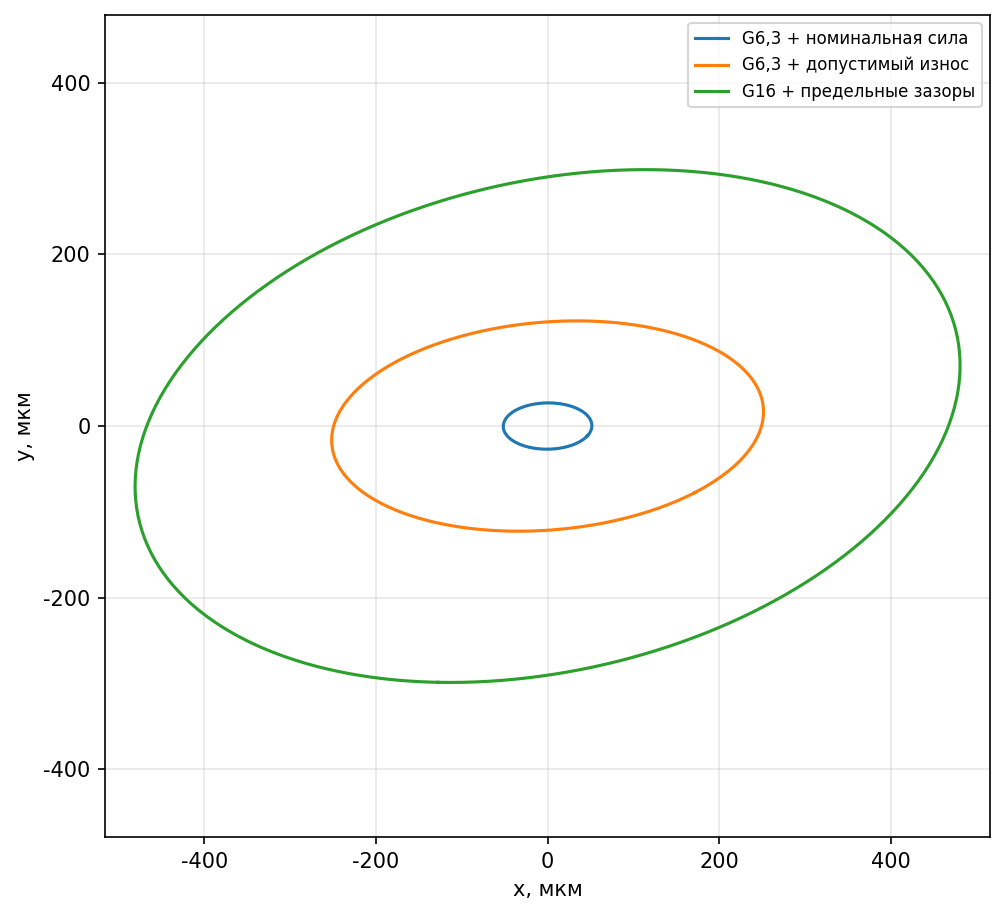
\includegraphics[width=0.75\textwidth]{09_orbits_comparison_seals.png}
\caption{Орбиты центрального сечения при разных эксплуатационных нагрузках}
\label{fig:orbits_center}
\end{figure}

В опорных сечениях влияние матрицы опоры выражено сильнее. На рисунке \ref{fig:support_orbits} показан предельно допустимый вариант G16 с повышенной гидравлической силой и увеличенными зазорами. В левой опоре полуоси составили $64{,}05$ и $5{,}46$ мкм, в правой -- $13{,}41$ и $1{,}48$ мкм. Максимальное отношение полуосей равно $11{,}74$, что подтверждает эллиптический характер движения.

\begin{figure}[H]
\centering

\includegraphics[width=0.75\textwidth]{16_support_orbits_full_matrix.png}
\caption{Орбиты в опорных сечениях для предельно допустимого варианта G16}
\label{fig:support_orbits}
\end{figure}

Полученные орбиты подтверждают, что движение в плоскостях $x$ и $y$ не является дублированием одной балочной модели. Эллиптичность связана с различием прямых коэффициентов $K_{xx}$, $K_{yy}$, наличием перекрёстных компонентов матрицы опоры и неравными проекциями эксплуатационной силы.

\subsection{Расчёт перекоса шейки}

По гармонической реакции ротора определены углы поворота опорных сечений. Для нового ротора с классом G6,3 и номинальной гидравлической силой максимальный угол перекоса составляет $0{,}098$ мрад. В предельно допустимом варианте G16 с повышенной гидравлической силой и увеличенными зазорами максимальный угол увеличивается до $0{,}840$ мрад.

На рисунке \ref{fig:mis_clearance} показано изменение минимального зазора вдоль длины вкладыша. При $\varepsilon=0{,}347$ зазор без перекоса составляет около $34{,}9$ мкм. Для предельно допустимого варианта минимальный краевой зазор равен $18{,}14$ мкм. Запас по зазору сохраняется, однако влияние перекоса становится заметным.

\begin{figure}[H]
\centering

\includegraphics[width=0.90\textwidth]{12_misalignment_clearance.png}
\caption{Влияние перекоса шейки на минимальный зазор вдоль вкладыша}
\label{fig:mis_clearance}
\end{figure}

На рисунке \ref{fig:mis_pressure} приведено распределение давления вдоль вкладыша в зоне максимального давления. В предельно допустимом варианте максимальное давление увеличивается с $0{,}685$ до $0{,}897$ МПа, то есть на $31{,}0\%$. Для выбранного режима это не приводит к потере работоспособности подшипника, но показывает направление влияния перекоса.

\begin{figure}[H]
\centering

\includegraphics[width=0.90\textwidth]{13_misalignment_pressure_axial.png}
\caption{Распределение давления вдоль вкладыша без перекоса и с перекосом}
\label{fig:mis_pressure}
\end{figure}

\subsection{Параметрические исследования}

На рисунке \ref{fig:sweep_eccentricity} показано влияние эксцентриситета на первую частотную ветвь. Увеличение эксцентриситета повышает жёсткость масляной плёнки и заметно увеличивает критическую скорость жёсткой оценки. Для упругой модели первая частотная ветвь практически не меняется: при изменении эксцентриситета от $0{,}20$ до $0{,}80$ она находится в узком диапазоне $1623$--$1634$ об/мин. Это связано с тем, что для длинного многоступенчатого ротора первая критическая скорость определяется преимущественно изгибной жёсткостью вала, а вклад опор является вторичным. Следовательно, расчёт без учёта упругости вала существенно завышает критическую скорость.

\begin{figure}[H]
\centering

\includegraphics[width=0.90\textwidth]{10_sweep_eccentricity.png}
\caption{Влияние эксцентриситета на первую частотную ветвь}
\label{fig:sweep_eccentricity}
\end{figure}

На рисунке \ref{fig:sweep_span} приведено влияние расстояния между опорами. При увеличении пролёта первая частотная ветвь упругой модели снижается, что соответствует росту изгибной податливости вала.

\begin{figure}[H]
\centering

\includegraphics[width=0.90\textwidth]{11_sweep_span.png}
\caption{Влияние расстояния между опорами на первую частотную ветвь}
\label{fig:sweep_span}
\end{figure}

На рисунке \ref{fig:sensitivity} показан анализ чувствительности модели к коэффициенту Ломакина $\lambda_L$ в диапазоне $\pm30\%$ от номинального значения. При изменении $\lambda_L$ от $0{,}385$ до $0{,}715$ первая частотная ветвь меняется от $3258{,}1$ до $4094{,}1$ об/мин, что соответствует отклонению от $-12{,}0$ до $+10{,}6\%$. Умеренный характер изменения показывает устойчивость результата к неопределённости коэффициента щелевого уплотнения.

\begin{figure}[H]
\centering

\includegraphics[width=0.90\textwidth]{14_sensitivity_lomakin_lambda.png}
\caption{Анализ чувствительности первой частотной ветви}
\label{fig:sensitivity}
\end{figure}


\subsection{Анализ устойчивости и нормативная оценка}

Проверка устойчивости выполнена по комплексным собственным значениям системы первого порядка. В таблице \ref{tab:stability_summary} приведены низшие собственные ветви для трёх эксплуатационных сценариев. Для нового ротора и варианта допустимого износа действительные части первых трёх ветвей отрицательны, поэтому свободные колебания в рабочем диапазоне затухают. Для предельно допустимого варианта G16 третья ветвь имеет $\operatorname{Re}(s_3)=6{,}91$ c$^{-1}$ и отрицательный логарифмический декремент $\delta_3=-0{,}053$, что указывает на потерю запаса устойчивости в расчётной низкочастотной области.

\begin{table}[H]
\centering
\small
\caption{Оценка устойчивости по собственным значениям}
\label{tab:stability_summary}
\begin{tabularx}{\textwidth}{>{\raggedright\arraybackslash}Xrrrr>{\raggedright\arraybackslash}X}
\toprule
Сценарий & $n_1$, об/мин & $\operatorname{Re}(s_1)$, c$^{-1}$ & $\delta_1$ & $\min\delta_{1..3}$ & Вывод \\
\midrule
G6,3, номинальный режим & 3701{,}8 & -46{,}70 & 0{,}757 & 0{,}504 & устойчив, запас по декременту достаточный \\
G6,3, допустимый износ & 3197{,}3 & -34{,}01 & 0{,}638 & 0{,}138 & устойчив, запас по декременту близок к нижней границе \\
G16, предельные зазоры & 2900{,}0 & -19{,}35 & 0{,}400 & -0{,}053 & динамический запас потерян по третьей ветви \\
\bottomrule
\end{tabularx}
\end{table}

На рисунке \ref{fig:log_decrement} показано изменение логарифмического декремента. Первая ветвь остаётся затухающей во всех вариантах, однако минимум по первым трём ветвям снижается от $0{,}504$ в номинальном режиме до отрицательного значения в предельном состоянии. В качестве практического критерия принято условие $\delta\geq0{,}1$, применяемое в ротородинамических проверках по API 684 [13].

\begin{figure}[H]
\centering

\includegraphics[width=0.88\textwidth]{17_log_decrement_stability.png}
\caption{Логарифмический декремент затухания для эксплуатационных сценариев}
\label{fig:log_decrement}
\end{figure}

Для практической интерпретации результаты сопоставлены с нормативными критериями. Для центробежных насосов по API 610 / ISO 13709 рабочая частота должна быть удалена от критических скоростей не менее чем на $15$--$20\%$ [19]. Вибрационная оценка выполнена по ГОСТ Р ИСО 20816 и ISO 20816 для среднеквадратичной виброскорости в опорных сечениях: зоны A/B/C/D используются как укрупнённая шкала состояния машины [20]. Так как расчётная орбита является перемещением вала, виброскорость определялась по максимальной полуоси орбиты в опорном сечении:
\begin{equation}
    v_{\text{rms}}=\frac{a\Omega}{\sqrt{2}},
    \label{eq:rms_velocity_from_orbit}
\end{equation}
где $a$ -- большая полуось орбиты, м. Для шкалы зон приняты границы: A -- до $2{,}3$ мм/с, B -- до $4{,}5$ мм/с, C -- до $7{,}1$ мм/с, D -- свыше $7{,}1$ мм/с.

\begin{table}[H]
\centering
\small
\caption{Сравнение эксплуатационных сценариев с нормативными критериями}
\label{tab:normative_summary}
\begin{tabularx}{\textwidth}{>{\raggedright\arraybackslash}Xrrrr>{\raggedright\arraybackslash}X}
\toprule
Сценарий & Запас до $n_1$, \% & $a_{\text{оп}}$, мкм & $v_{\text{rms}}$, мм/с & Зона & Практический вывод \\
\midrule
G6,3, номинальный режим & 25{,}5 & 2{,}14 & 0{,}47 & A & запас по критической скорости и вибрации достаточен \\
G6,3, допустимый износ & 8{,}4 & 26{,}32 & 5{,}75 & C & необходим контроль зазоров и вибрации, длительная работа нежелательна \\
G16, предельные зазоры & 1{,}7 & 64{,}05 & 13{,}99 & D & состояние близко к резонансу и требует вывода в ремонт \\
\bottomrule
\end{tabularx}
\end{table}

Из таблицы \ref{tab:normative_summary} следует, что новый ротор имеет достаточный частотный запас: первая ветвь находится на $25{,}5\%$ выше рабочей частоты $2950$ об/мин. При допустимом износе первая ветвь снижается до $3197{,}3$ об/мин, запас уменьшается до $8{,}4\%$, поэтому эксплуатация требует контроля вибрации и зазоров. В предельном варианте G16 первая ветвь $2900{,}0$ об/мин находится практически на рабочей частоте; одновременно виброскорость попадает в зону D, а третья собственная ветвь имеет отрицательный декремент. Практически это означает необходимость балансировки ротора, контроля щелевых уплотнений и восстановления зазоров подшипников при ремонте.

\subsection{Сравнение расчётных вариантов}

Сравнение вариантов показывает, что динамические характеристики ротора существенно зависят от состояния зазоров и уровня остаточного дисбаланса. Номинальный вариант удовлетворяет критерию удаления от первой критической скорости и имеет положительный логарифмический декремент. При допустимом износе устойчивость первых ветвей сохраняется, однако запас до первой критической скорости становится недостаточным. Предельный вариант G16 с увеличенными зазорами оказывается близким к рабочей скорости и одновременно теряет запас устойчивости по третьей ветви. Учёт гидравлической радиальной силы потока и допустимого износа приводит к орбитам в диапазоне десятков и сотен микрометров, что соответствует инженерно наблюдаемому уровню смещений секционного насоса.

Результаты также показывают важность использования реальных массовых характеристик рабочих колёс. Суммарная масса колёс ЦНС 105-392 по расчётной схеме составляет $131{,}6$ кг; колесо первой ступени принято непосредственно по чертежу, а масса остальных колёс задана расчётно по спецификации. Индивидуальное распределение масс повышает достоверность матрицы масс и расчёта собственных форм.



\subsection{Выводы по третьей главе}

В третьей главе выполнен численный расчёт динамических характеристик ротора насоса ЦНС 105-392. Массовая схема построена по спецификации сборочного чертежа: колесо первой ступени имеет массу $19{,}6$ кг по чертежу ЦНС 90.00.00.012, остальные семь рабочих колёс учтены расчётной массой $16{,}0$ кг. Суммарная масса рабочих колёс составляет $131{,}6$ кг, а полная расчётная масса ротора с валом -- $229{,}03$ кг.

Статическое равновесие ротора дало реакции $W_1=1{,}185$ кН и $W_2=1{,}062$ кН. По зависимости несущей способности масляной плёнки от эксцентриситета получены рабочие положения шейки: $\varepsilon_1=0{,}360$ для левой опоры и $\varepsilon_2=0{,}334$ для правой. Таким образом, эксцентриситет подшипника является результатом расчёта равновесия, а не назначенным параметром.

По модели гладкого подшипника при среднем рабочем эксцентриситете $\varepsilon=0{,}347$ получено максимальное давление $0{,}685$ МПа, несущая сила $1{,}102$ кН и минимальный зазор $34{,}95$ мкм. Для базового режима матрица опоры имеет выраженные перекрёстные компоненты: $K_{xx}=5{,}55\cdot10^7$ Н/м, $K_{yy}=2{,}25\cdot10^7$ Н/м, $K_{xy}=5{,}46\cdot10^7$ Н/м и $K_{yx}=-7{,}36\cdot10^7$ Н/м.

Комплексный расчёт собственных частот показал разделение первой пары на ветви прямой и обратной прецессии. Без щелевых уплотнений первая пара равна $1629{,}3$ и $1634{,}2$ об/мин. При учёте щелевых уплотнений первая пара повышается до $3701{,}8$ и $3705{,}7$ об/мин. Для варианта допустимого износа первая ветвь снижается до $3197{,}3$ об/мин, а для предельно допустимого варианта G16 с увеличенными зазорами -- до $2900{,}0$ об/мин, то есть оказывается близкой к рабочей скорости $2950$ об/мин.

Расчёт орбит с эксплуатационными нагрузками дал инженерно значимые амплитуды. Для нового ротора G6,3 с номинальной гидравлической силой полуоси орбиты центрального сечения составляют $51{,}60$ и $26{,}95$ мкм. Для варианта допустимого износа полуоси возрастают до $252{,}20$ и $121{,}03$ мкм, а для предельно допустимого варианта G16 -- до $488{,}38$ и $285{,}49$ мкм. В опорных сечениях орбиты имеют эллиптическую форму с отношением полуосей до $11{,}74$, что отражает анизотропию и перекрёстные коэффициенты подшипника.

Анализ устойчивости показал, что в номинальном режиме первая ветвь имеет $\operatorname{Re}(s_1)=-46{,}70$ c$^{-1}$ и $\delta_1=0{,}757$, а минимальный декремент первых трёх ветвей равен $0{,}504$. При допустимом износе минимальный декремент снижается до $0{,}138$, но остаётся выше ориентировочного критерия $0{,}1$. В предельном варианте G16 третья ветвь имеет $\operatorname{Re}(s_3)=6{,}91$ c$^{-1}$ и $\delta_3=-0{,}053$, поэтому динамический запас считается потерянным. Нормативное сопоставление показало: новый ротор имеет запас по критической скорости $25{,}5\%$ и зону вибрации A в опорном сечении; при допустимом износе запас снижается до $8{,}4\%$ и виброскорость переходит в зону C; в предельном состоянии запас составляет только $1{,}7\%$, а виброскорость соответствует зоне D.

Гидравлическая радиальная сила, рассчитанная по реальным параметрам колеса $D_2=0{,}300$ м и $B_2=0{,}0224$ м, составляет $516{,}8$ Н на номинальном режиме и $1033{,}7$ Н на нерасчётном режиме. Допустимый дисбаланс по чертежу $D_b=250$ г$\cdot$мм даёт силу $23{,}86$ Н, что совпадает по порядку с оценкой по классу G6,3. Анализ чувствительности к коэффициенту Ломакина показал изменение первой частотной ветви от $-12{,}0$ до $+10{,}6\%$ при изменении $\lambda_L$ на $\pm30\%$, поэтому результат устойчив к разумной неопределённости параметров щелевых уплотнений.

\newpage
\section*{Список использованных источников}
\addcontentsline{toc}{section}{Список использованных источников}


\begin{enumerate}
    \item ТУ 3631-003-00217389-96. Насосы центробежные секционные типа ЦНС. Технические условия.
    \item ГОСТ 31381-2009. Насосы динамические. Методы испытаний. Москва: Стандартинформ, 2010.
    \item Сборочный чертёж насоса ЦНС 105-392 (5МС-10) и чертёж опорного подшипника скольжения. Комплект конструкторской документации кафедры ТМиО НГК, УГНТУ.
    \item ГОСТ 801-78. Сталь подшипниковая. Технические условия. Москва: Издательство стандартов, 1978.
    \item Колесо рабочее 1 ступени ЦНС 90.00.00.012. Чертёж детали, УГНТУ МП-98-02.
    \item Mota J. A., Maldonado D. J. G., Valério J. V., Ritto T. G. Complete modeling of hydrodynamic bearings with a boundary parameterization approach // Mechanism and Machine Theory. 2021. Vol. 162. Article 104350.
    \item Ломакин А. А. Расчёт критического числа оборотов и условий обеспечения динамической устойчивости роторов гидравлических машин высокого давления с учётом сил в уплотнениях // Энергомашиностроение. 1958. № 4. С. 1--8.
    \item Ломакин А. А. Центробежные и осевые насосы. 2-е изд., перераб. и доп. Москва; Ленинград: Машиностроение, 1966. 364 с.
    \item Black H. F., Jenssen D. N. Dynamic hybrid bearing characteristics of annular controlled leakage seals // Proceedings of the Institution of Mechanical Engineers. 1969. Vol. 184. P. 92--100.
    \item Hirs G. G. A bulk-flow theory for turbulence in lubricant films // Journal of Lubrication Technology. 1973. Vol. 95, no. 2. P. 137--146.
    \item Childs D. W. Turbomachinery Rotordynamics: Phenomena, Modeling, and Analysis. New York: Wiley, 1993.
    \item San Andrés L. Analysis of turbulent annular seals with fluid inertia effects // ASME Journal of Tribology. 1991. Vol. 113. P. 302--309.
    \item API Recommended Practice 684. API Standard Paragraphs Rotordynamic Tutorial: Lateral Critical Speeds, Unbalance Response, Stability, Train Torsionals, and Rotor Balancing. 4th ed. Washington: American Petroleum Institute, 2014. Reaffirmed 2022.
    \item ГОСТ ИСО 1940-1-2007. Вибрация. Требования к качеству балансировки жёстких роторов. Часть 1. Определение допустимого остаточного дисбаланса. Москва: Стандартинформ, 2008.
    \item Степанов А. И. Центробежные и осевые насосы. Москва: Машгиз, 1960.
    \item Xiong G., Zhang J., Mao Z., Wang Z., Wang H., Lian S., Jiang Z. Dynamic misalignment effects on performance of dynamically loaded journal bearings // International Journal of Mechanical Sciences. 2024. Vol. 264. Article 108839.
    \item Gu C., Meng X., Wang S., Ding X. Modeling a hydrodynamic bearing with provision for misalignments and textures // Journal of Tribology. 2020. Vol. 142. Article 041801.
    \item Xie Z., Jiao J., Zhao B., Zhang J., Xu F. Theoretical and experimental research on the effect of bi-directional misalignment on the static and dynamic characteristics of a novel bearing // Mechanical Systems and Signal Processing. 2024. Vol. 208. Article 111041.
    \item API Standard 610. Centrifugal Pumps for Petroleum, Petrochemical and Natural Gas Industries. 12th ed. Washington: American Petroleum Institute, 2021; ISO 13709:2009. Centrifugal pumps for petroleum, petrochemical and natural gas industries. Geneva: ISO, 2009.
    \item ГОСТ Р ИСО 20816-3-2023. Вибрация. Измерение и оценка вибрации машин. Часть 3. Машины промышленного назначения номинальной мощностью более 15 кВт и номинальными скоростями от 120 об/мин до 30000 об/мин. Москва: Стандартинформ, 2023.
\end{enumerate}

\end{document}
